\documentclass[11pt]{article}
\usepackage[margin=0.78in]{geometry}
\usepackage[T1]{fontenc}
\usepackage{lmodern}
\usepackage{microtype}
\usepackage{booktabs,longtable,array,tabularx,graphicx,pdflscape}
\usepackage{xcolor,enumitem}
\usepackage{tikz}
\usetikzlibrary{arrows.meta,positioning,shapes.geometric,fit}
\usepackage[hidelinks]{hyperref}
\hypersetup{pdftitle={Relay System Design Document},pdfauthor={Relay Capstone Team},colorlinks=true,linkcolor=blue!55!black,urlcolor=blue!55!black}
\setlength{\parindent}{0pt}
\setlength{\parskip}{0.55em}
\setlist{nosep,leftmargin=*}
\renewcommand{\arraystretch}{1.18}
\newcommand{\implemented}{\textbf{Implemented}}
\newcommand{\partialstatus}{\textbf{Partial}}
\newcommand{\unverified}{\textbf{Unverified}}

\title{\textbf{Relay System Design Document}\\
\large AI-Assisted Email, Calendar, Memory, and Workflow Platform}
\author{Dhruv Mann --- \texttt{dmann9@myseneca.ca}\\
Arshia Barootkoob Dezfooli --- \texttt{abarootkoob-dezfooli@myseneca.ca}\\
Dipak Prasad Kushwaha --- \texttt{dkushwaha@myseneca.ca}\\
Smeet Brijesh Patel --- \texttt{spatel577@myseneca.ca}\\[0.6em]
Instructor: Miguel Watler --- \texttt{miguel.watler@senecapolytechnic.ca}\\
SED800 --- Seneca Polytechnic}
\date{Implementation and test baseline: August 11, 2026}

\begin{document}
\maketitle

\begin{abstract}
This document records Relay's original requirements, implemented architecture,
design evolution, low-level flows, data model, alternatives, trust boundaries,
and remaining design debt. It is evidence-based. Implemented means repository
code and automated evidence exist; partial means a useful foundation exists but
a planned behavior or live validation is missing; and unverified means the
original target lacks sufficient baseline evidence. This source is intended to
be published with the Relay repository and linked from the capstone thesis.
\end{abstract}

\tableofcontents
\newpage

\section{Purpose, Scope, and Evidence}

Relay unifies Gmail and Outlook with AI-assisted summaries and drafts,
calendar and commitment workflows, reviewable memory, semantic context, and
durable activity history. The design preserves provider differences,
authenticates every user-owned operation, keeps credentials server-side,
isolates data by user/account, and degrades safely when dependencies fail.

Evidence sources:
\begin{itemize}
  \item Repository: \url{https://github.com/dmann001/Relay-agent-back}
  \item Changelog: \url{https://github.com/dmann001/Relay-agent-back/blob/main/docs/CHANGELOG.md}
  \item QA: \url{https://github.com/dmann001/Relay-agent-back/blob/main/docs/QA.md}
  \item Memory: \url{https://github.com/dmann001/Relay-agent-back/blob/main/docs/MEMORY_ARCHITECTURE.md}
  \item Security: \url{https://github.com/dmann001/Relay-agent-back/blob/main/docs/Relay_Security_Plan.pdf}
\end{itemize}
Public links must be tested while signed out before submission.

\section{Requirements and Evolution}

The original project-plan requirements are retained so changes are traceable.

\subsection{Functional Requirements}

\begin{longtable}{@{}p{0.06\textwidth}p{0.25\textwidth}p{0.39\textwidth}p{0.20\textwidth}@{}}
\toprule
ID & Original requirement & End-product implementation & Status/evolution \\
\midrule
\endhead
\bottomrule
\endlastfoot
FR-01 & Gmail/Outlook OAuth 2.0 & Supabase user authentication plus provider callbacks and encrypted tokens & \implemented; identity and delegation separated \\
FR-02 & Multiple account management & Account records, selector, scoped APIs, disconnect behavior & \implemented \\
FR-03 & Synchronize connected accounts & Gmail history and Outlook delta synchronization & \implemented; cursor pulls replaced webhook dependencies \\
FR-04 & Unified inbox & Shared routes and provider-neutral records & \implemented \\
FR-05 & Complete thread view & Provider-aware message/thread routes & \implemented \\
FR-06 & AI summaries & Thread assistant and brief routes & \implemented; semantic evaluation pending \\
FR-07 & Context-aware drafts & Preferences, contact context, memory, selected email & \implemented \\
FR-08 & Full-text and vector search & Provider search plus semantic personalization chunks & \partialstatus; unified FTS/vector endpoint absent \\
FR-09 & RAG with citations & Same-contact history, memory, semantic chunks, exact selected threads & \partialstatus; generalized grounding/fallback and citations incomplete \\
FR-10 & Agent proposals & Calendar, commitments, monitors, briefs, activity & \partialstatus; generic proposal/label tool absent \\
FR-11 & Explicit confirmation & Activity states plus owned cancel/retry & \partialstatus; approve/claim/revalidate/execute required \\
FR-12 & Embedding storage & pgvector chunks, match function, hashes, indexes & \implemented; production recall/scale unverified \\
FR-13 & RLS isolation & Ownership columns, RLS SQL, constraints, contracts & \partialstatus until deployed two-user test \\
\end{longtable}

\subsection{Non-Functional Requirements}

\begin{longtable}{@{}p{0.07\textwidth}p{0.25\textwidth}p{0.40\textwidth}p{0.18\textwidth}@{}}
\toprule
ID & Original group & End-product design/evidence & Status/evolution \\
\midrule
\endhead
\bottomrule
\endlastfoot
NFR-01 & Security & AES-256-GCM, OAuth, ownership, RLS SQL, validation, security plan & \partialstatus; deployed headers/RLS, legacy isolation, pen test needed \\
NFR-02 & Reliability & Token refresh, Gmail recovery, Outlook delta, soft AI failure, activity events & \partialstatus; monitoring, backup, failure injection incomplete \\
NFR-03 & Performance & Pagination, provider limits, regression tests, indexes & \unverified against numeric targets \\
NFR-04 & Scalability & Modular monolith, multi-account schema, cursor/vector indexes & Foundation implemented; capacity unverified \\
NFR-05 & Privacy & Server credentials, bounded context, user-owned memory, OpenAI disclosure & \partialstatus; third-party wording corrected; retention incomplete \\
NFR-06 & Usability & Responsive navigation, feedback states, assistants, settings, activity UI & \partialstatus until accessibility/user testing \\
\end{longtable}

\section{Design Evolution}

\begin{longtable}{@{}p{0.15\textwidth}p{0.24\textwidth}p{0.27\textwidth}p{0.24\textwidth}@{}}
\toprule
Concern & Original design & Implemented end product & Reason/consequence \\
\midrule
\endhead
\bottomrule
\endlastfoot
Web boundary & React SPA and Express REST API & Next.js pages/routes; legacy Express remains & Reduced CORS, session, routing, deployment complexity \\
Provider sync & Gmail watch/history and Graph webhooks/delta & Gmail history pulls and Outlook delta pulls & Incremental sync without webhook infrastructure \\
Model providers & OpenAI and Anthropic & OpenAI Responses and Embeddings & Reduced adapter/evaluation scope \\
Search & Database FTS plus vectors & Provider search plus semantic personalization chunks & Provider-accurate search shipped; unified local search partial \\
RAG & Message/attachment embeddings and citations & Selected threads, same-contact mail, memory, message chunks & Attachment RAG and auto-grounding remain future work \\
Agent layer & Generic proposals with confirmation & Calendar/commitments, monitors, briefs, activity, cancel/retry & Concrete workflows shipped before approval executor \\
Data model & Core mail, embeddings, tasks & Provider-neutral mail plus memory, calendars, commitments, briefs, activity & Scope expanded into a communication workspace \\
Privacy & Never share with third parties & Minimized context sent to configured OpenAI service & Incompatible wording corrected; transparency required \\
\end{longtable}

\section{High-Level Architecture}

\begin{figure}[htbp]
\centering
\resizebox{\textwidth}{!}{%
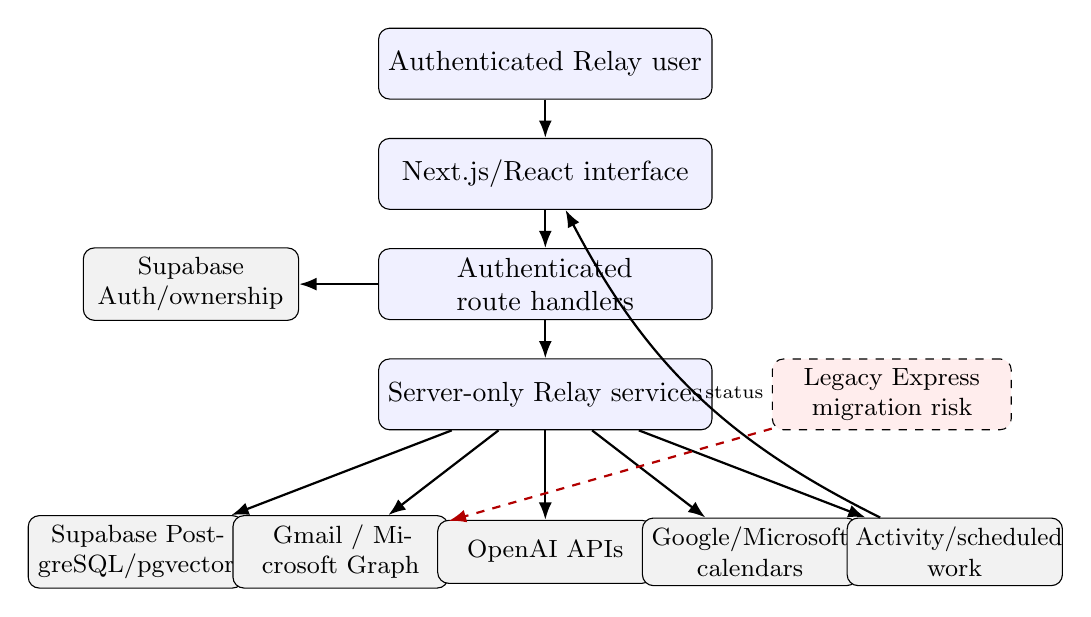
\begin{tikzpicture}[
  >={Latex[length=2.2mm]},
  box/.style={draw,rounded corners,fill=blue!6,align=center,minimum height=0.9cm,text width=4.0cm},
  service/.style={draw,rounded corners,fill=gray!10,align=center,minimum height=0.8cm,text width=2.5cm,font=\small},
  risk/.style={draw,dashed,rounded corners,fill=red!7,align=center,text width=2.8cm,font=\small}
]
\node[box] (user) at (0,4.2) {Authenticated Relay user};
\node[box] (ui) at (0,2.8) {Next.js/React interface};
\node[box] (api) at (0,1.4) {Authenticated route handlers};
\node[service] (auth) at (-4.5,1.4) {Supabase Auth/ownership};
\node[box] (core) at (0,0) {Server-only Relay services};
\node[service] (db) at (-5.2,-2.0) {Supabase PostgreSQL/pgvector};
\node[service] (mail) at (-2.6,-2.0) {Gmail / Microsoft Graph};
\node[service] (ai) at (0,-2.0) {OpenAI APIs};
\node[service] (cal) at (2.6,-2.0) {Google/Microsoft calendars};
\node[service] (activity) at (5.2,-2.0) {Activity/scheduled work};
\node[risk] (legacy) at (4.4,0) {Legacy Express migration risk};
\foreach \a/\bb in {user/ui,ui/api,api/core,api/auth,core/db,core/mail,core/ai,core/cal,core/activity}
  \draw[->,thick] (\a) -- (\bb);
\draw[->,thick,bend left=18] (activity) to node[right,font=\scriptsize]{status} (ui);
\draw[->,thick,dashed,red!70!black] (legacy) -- (mail);
\end{tikzpicture}}
\caption{Implemented architecture and principal trust boundaries.}
\end{figure}

The browser is untrusted. Routes authenticate the user, resolve account
ownership, validate input, and call server-only modules. Provider tokens,
service-role credentials, OAuth/cron secrets, encryption keys, and OpenAI keys
remain server-side. Mail, model output, and memory candidates are data, not authority.

\subsection{Component Responsibilities}

\begin{longtable}{@{}p{0.20\textwidth}p{0.35\textwidth}p{0.35\textwidth}@{}}
\toprule
Component & Responsibility & Main implementation surface \\
\midrule
\endhead
\bottomrule
\endlastfoot
Web interface & Account scope, mailbox/thread/compose, assistants, calendar, commitments, activity, settings & \texttt{app}, \texttt{components}, \texttt{lib/email-api.ts} \\
Authentication/accounts & Relay identity, OAuth state, token lifecycle, ownership & auth routes, provider account modules, \texttt{crypto.ts} \\
Provider adapters & Fetch, sync, search, thread, draft, send, modify & Gmail/Outlook API and sync modules \\
AI/context & Structured output, rate limits, selected-thread and personalization context & AI routes, \texttt{openai.ts}, \texttt{personalization.ts} \\
Memory & Quality filters, review, feedback, semantic chunks, maintenance & memory routes and server memory modules \\
Workflow & Commitments, monitors, calendars, briefs, activity/events & workflow routes, \texttt{agent-activity.ts} \\
Data layer & Relational records, RLS, constraints, indexes, migrations & \texttt{supabase/schema.sql}, migrations \\
\end{longtable}

\section{Data Design}

Every primary domain row carries \texttt{user\_id} or derives ownership from an
owned parent. Provider identifiers remain beside normalized records. Uniqueness
on account/provider identifiers prevents duplicates. RLS is defense in depth;
service-role routes must still authenticate and filter.

\begin{landscape}
\begin{figure}[p]
\centering
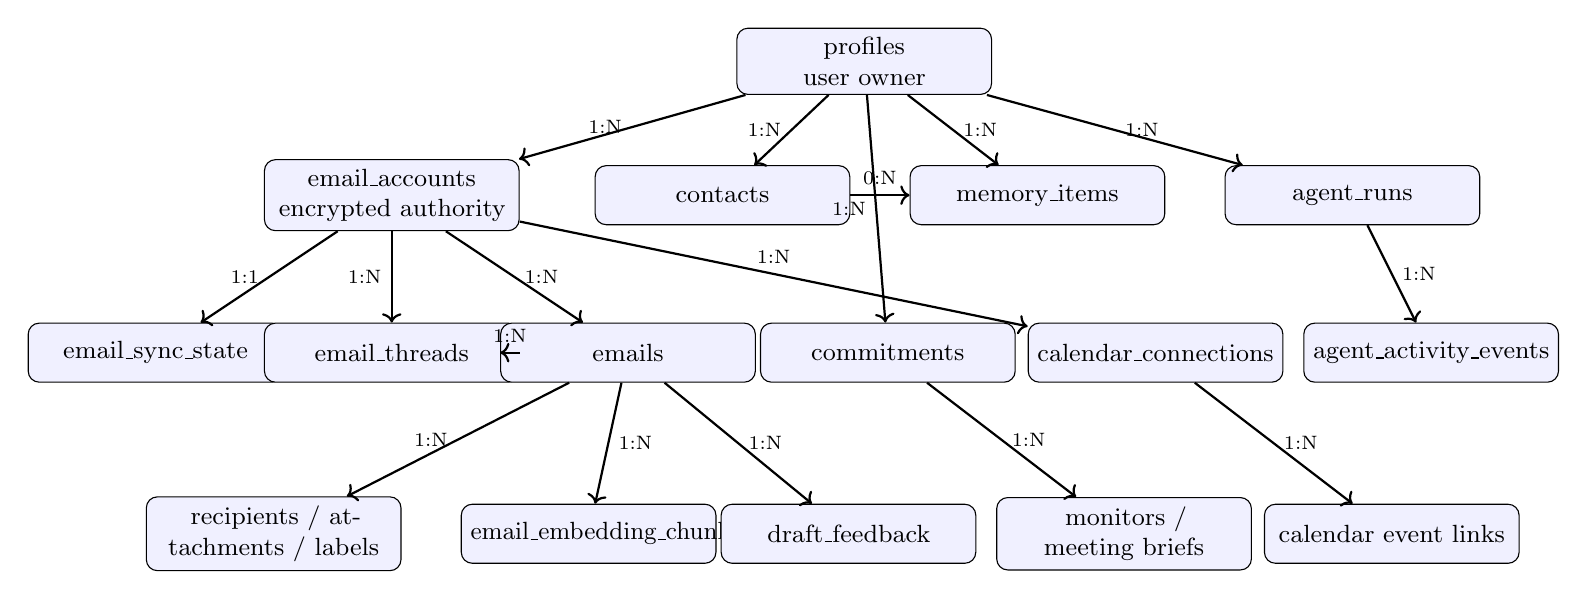
\begin{tikzpicture}[
  entity/.style={draw,rounded corners,fill=blue!6,align=center,minimum height=0.75cm,text width=3.0cm,font=\small},
  rel/.style={draw,->,thick,font=\scriptsize}
]
\node[entity] (profile) at (0,6) {profiles\\user owner};
\node[entity] (account) at (-6,4.3) {email\_accounts\\encrypted authority};
\node[entity] (contact) at (-1.8,4.3) {contacts};
\node[entity] (memory) at (2.2,4.3) {memory\_items};
\node[entity] (runs) at (6.2,4.3) {agent\_runs};
\node[entity] (sync) at (-9,2.3) {email\_sync\_state};
\node[entity] (threads) at (-6,2.3) {email\_threads};
\node[entity] (emails) at (-3,2.3) {emails};
\node[entity] (commit) at (0.3,2.3) {commitments};
\node[entity] (cal) at (3.7,2.3) {calendar\_connections};
\node[entity] (events) at (7.2,2.3) {agent\_activity\_events};
\node[entity] (mailparts) at (-7.5,0) {recipients / attachments / labels};
\node[entity] (chunks) at (-3.5,0) {email\_embedding\_chunks};
\node[entity] (feedback) at (-0.2,0) {draft\_feedback};
\node[entity] (workflow) at (3.3,0) {monitors / meeting briefs};
\node[entity] (links) at (6.7,0) {calendar event links};
\draw[rel] (profile) -- node[left]{1:N} (account);
\draw[rel] (profile) -- node[left]{1:N} (contact);
\draw[rel] (profile) -- node[right]{1:N} (memory);
\draw[rel] (profile) -- node[right]{1:N} (runs);
\draw[rel] (account) -- node[left]{1:1} (sync);
\draw[rel] (account) -- node[left]{1:N} (threads);
\draw[rel] (account) -- node[right]{1:N} (emails);
\draw[rel] (threads) -- node[above]{1:N} (emails);
\draw[rel] (emails) -- node[left]{1:N} (mailparts);
\draw[rel] (emails) -- node[right]{1:N} (chunks);
\draw[rel] (emails) -- node[right]{1:N} (feedback);
\draw[rel] (profile) -- node[left]{1:N} (commit);
\draw[rel] (commit) -- node[right]{1:N} (workflow);
\draw[rel] (account) -- node[above]{1:N} (cal);
\draw[rel] (cal) -- node[right]{1:N} (links);
\draw[rel] (runs) -- node[right]{1:N} (events);
\draw[rel] (contact) -- node[above]{0:N} (memory);
\end{tikzpicture}
\caption{Core logical ER model. Settings and minor auxiliary tables are omitted.}
\end{figure}
\end{landscape}

\section{Low-Level Interaction Design}

\subsection{OAuth Connection Sequence}

\begin{figure}[htbp]
\centering
\resizebox{\textwidth}{!}{%
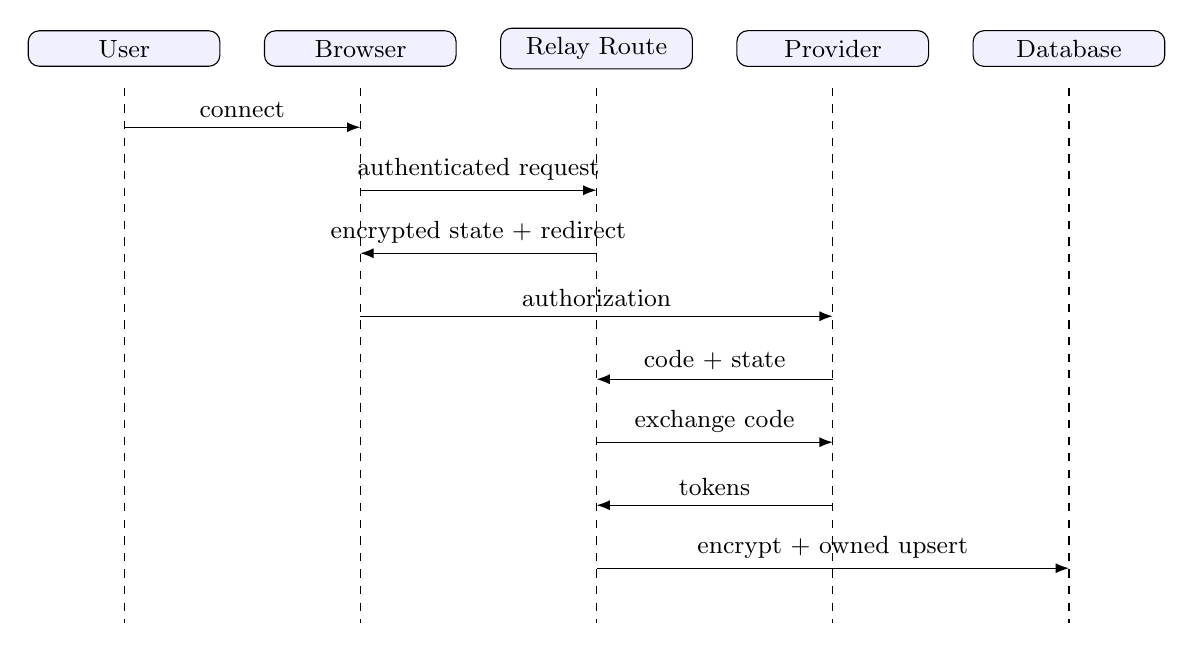
\begin{tikzpicture}[>=Latex,font=\small]
\foreach \x/\name in {0/User,3/Browser,6/Relay Route,9/Provider,12/Database}{
  \node[draw,rounded corners,fill=blue!6,text width=2.2cm,align=center] at (\x,0) {\name};
  \draw[dashed] (\x,-0.5) -- (\x,-7.3);
}
\draw[->] (0,-1) -- node[above]{connect} (3,-1);
\draw[->] (3,-1.8) -- node[above]{authenticated request} (6,-1.8);
\draw[->] (6,-2.6) -- node[above]{encrypted state + redirect} (3,-2.6);
\draw[->] (3,-3.4) -- node[above]{authorization} (9,-3.4);
\draw[->] (9,-4.2) -- node[above]{code + state} (6,-4.2);
\draw[->] (6,-5.0) -- node[above]{exchange code} (9,-5.0);
\draw[->] (9,-5.8) -- node[above]{tokens} (6,-5.8);
\draw[->] (6,-6.6) -- node[above]{encrypt + owned upsert} (12,-6.6);
\end{tikzpicture}}
\caption{Gmail/Outlook OAuth sequence; invalid or expired state terminates the callback.}
\end{figure}

\subsection{Synchronization Flows}

\begin{longtable}{@{}p{0.18\textwidth}p{0.52\textwidth}p{0.20\textwidth}@{}}
\toprule
Flow & Sequence & Safeguard \\
\midrule
\endhead
\bottomrule
\endlastfoot
Gmail & Resolve account; refresh; history cursor; fetch changes; unique upsert; update sync state & History expiry triggers bounded recovery \\
Outlook & Resolve account; refresh; delta page; normalize additions/removals; persist link & Cursor/removal account-scoped \\
Listing & Query cache using cursor indexes; determine provider pages; fetch bounded pages & Avoids whole-mailbox loads; omits tokens \\
\end{longtable}

\subsection{AI and Personalization Flow}

\begin{enumerate}
  \item Authenticate and resolve an owned account.
  \item Fetch the exact selected provider thread when referenced.
  \item Assemble preferences, accepted memory, contact data, same-contact sent
        mail, commitments, and optional semantic chunks.
  \item Bound each source and treat provider/model text as untrusted data.
  \item Call OpenAI server-side and validate structured output with Zod.
  \item Return the result and context-source categories without secrets.
  \item After provider send succeeds, filter/store draft feedback or a pending memory suggestion.
\end{enumerate}

The semantic path does not yet automatically re-fetch every vector match,
combine database FTS/vectors in one ranking, or fall back to provider search.

\subsection{Current Activity and Target Approval State}

\begin{figure}[htbp]
\centering
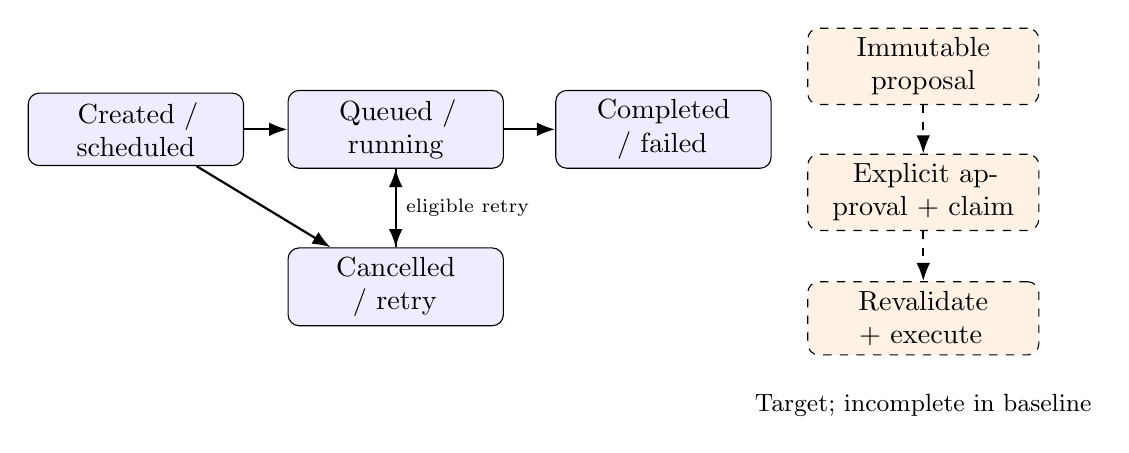
\begin{tikzpicture}[
  >={Latex},
  state/.style={draw,rounded corners,fill=blue!7,align=center,text width=2.5cm,minimum height=0.8cm},
  target/.style={draw,dashed,rounded corners,fill=orange!10,align=center,text width=2.7cm,minimum height=0.8cm}
]
\node[state] (created) at (-5,2) {Created / scheduled};
\node[state] (running) at (-1.7,2) {Queued / running};
\node[state] (done) at (1.7,2) {Completed / failed};
\node[state] (cancel) at (-1.7,0) {Cancelled / retry};
\draw[->,thick] (created) -- (running);
\draw[->,thick] (running) -- (done);
\draw[->,thick] (created) -- (cancel);
\draw[->,thick] (running) -- (cancel);
\draw[->,thick] (cancel) -- node[right,font=\scriptsize]{eligible retry} (running);
\node[target] (proposal) at (5,2.8) {Immutable proposal};
\node[target] (approve) at (5,1.2) {Explicit approval + claim};
\node[target] (execute) at (5,-0.4) {Revalidate + execute};
\draw[->,thick,dashed] (proposal) -- (approve);
\draw[->,thick,dashed] (approve) -- (execute);
\node[font=\small,align=center] at (5,-1.5) {Target; incomplete in baseline};
\end{tikzpicture}
\caption{Implemented activity lifecycle (solid) and target approval executor (dashed).}
\end{figure}

\section{Alternative Designs}

\begin{longtable}{@{}p{0.22\textwidth}p{0.30\textwidth}p{0.38\textwidth}@{}}
\toprule
Decision & Rejected/limited alternative & Selected direction \\
\midrule
\endhead
\bottomrule
\endlastfoot
Application & Separate SPA/public Express API expands CORS, deployment, session surfaces & Next.js backend-for-frontend; retire legacy Express \\
Topology & Microservices require service auth, tracing, queues, operations & Modular monolith; extract after measured need \\
Mailbox data & Provider-only increases latency; full mirror expands privacy burden & Bounded normalized cache plus provider truth \\
AI context & Single-shot prompts miss history/expose excessive context & Task-specific structured routes and bounded scope \\
Actions & Autonomous writes create authorization risk & User-directed writes now; approval executor before model writes \\
Memory & Broad graph complicates provenance/correction & Scoped ledger with state, evidence, confidence, expiry \\
\end{longtable}

\section{Security and Testing in the Design}

\subsection{Implemented Controls}
\begin{itemize}
  \item Supabase user validation and server-injected ownership.
  \item AES-256-GCM token and OAuth-state protection.
  \item RLS SQL, ownership constraints, uniqueness, and schema contracts.
  \item Zod validation, AI rate limits, MIME/header tests, HTML sanitization
        support, and bounded pagination.
  \item User-scoped memory with confidence, sensitivity, evidence, status,
        expiry, contradiction, correction, and deletion.
  \item User-owned activity and cancel/retry state validation.
\end{itemize}

\subsection{Required Completion}
\begin{itemize}
  \item Remove or isolate legacy Express routes.
  \item Verify deployed RLS with two users and several provider accounts.
  \item Verify HTTPS/security headers, retention/deletion, monitoring, backup,
        restore, incident response, and key rotation.
  \item Implement immutable, expiring, idempotent approval execution before
        consequential model proposals.
  \item Conduct injection, cross-account, replay, SSRF, leakage, and manual
        penetration tests in isolated staging.
\end{itemize}

Unit tests cover parsers, adapters, encryption, auth helpers, rate limits,
memory quality, personalization, pagination, and URL restrictions. Component
and integration tests cover UI, route authentication, ownership, normalization,
structured outputs, and activity states. Schema contracts inspect RLS and
constraints. Playwright, live providers, performance, accessibility, user
studies, and penetration testing require final evidence.

\section{Deployment Model}

The intended deployment is one primary Next.js application connected to
Supabase and external Gmail, Microsoft Graph, calendar, and OpenAI APIs. A
cron-authenticated endpoint processes scheduled work. Secrets are server-only.
CI installs, lints, type-checks, tests with coverage, builds, runs browser
checks, audits dependencies, and performs CodeQL where enabled. Production
availability, capacity, recovery, and incident readiness are not claimed.

\section{Completion Criteria}

\begin{enumerate}
  \item Complete database FTS/vector ranking, exact candidate grounding,
        provider fallback, citations, and recall/latency evaluation.
  \item Complete immutable approval payload, expiry, ownership, atomic claim,
        idempotency, revalidation, execution, and audit.
  \item Close security blockers and publish re-test evidence.
  \item Benchmark or formally revise the original latency targets.
  \item Validate accessibility, usability, multi-user isolation, and live providers.
  \item Publish retention, logging, backup, monitoring, and incident procedures.
\end{enumerate}

\section{Public Traceability}

This document provides public high/low-level design evidence, requirement
evolution, architecture, components, ER relationships, OAuth/sync sequences,
workflow state, alternatives, testing/security hooks, and deployment design.
After commit to the public repository, its canonical URL is:

\url{https://github.com/dmann001/Relay-agent-back/blob/main/docs/Relay_System_Design_Document.tex}

\end{document}
